\documentclass[11pt,a4paper]{article}
\usepackage{amsmath}
\usepackage{amsfonts}
\usepackage{amssymb}
\usepackage{graphicx}
\usepackage{hyperref} %inserting urls
\usepackage{nameref}
\graphicspath{{Graphics/}} %Setting the graphicspath
\usepackage[utf8]{inputenc}
\usepackage[english]{babel}
\usepackage{lmodern}
% caption einr
\usepackage{caption}
\captionsetup{singlelinecheck=false,
	font=small,
	labelfont=bf,
	format=hang,
}
% Operators
\DeclareMathOperator*{\argmin}{argmin}
\DeclareMathOperator*{\argmax}{argmax}

\author{Sebastian Knigge}
\begin{document}

\section{Discussed models}

This section will introduce the reader into the two Topic modeling approaches which will be compared in this Thesis. The aim of both procedures is to assign one or more topics to different documents. Even if the vocabulary and the notation are similar for both approaches, the notation should be resumed at the beginning of the description of the respective model. The basic structural notation of the data consists of the following variables.

A collection of documents is called corpus $D=(\textbf{w}_1,\dots , \textbf{w}_M)$. It consists out of M documents $\textbf{w}=(w_1,\dots, w_N)$ which are itself separated in words $w_i$. These words are vectors of length $V$. $V$ refers to the length of a vocabulary which holds all the words occurring in the corpus. The vector for a specific word $w_i$ contains all 0 except for index $j\in\{1,...,V\}$ which represents this very one word in the vocabulary.
This notation may indeed be extended through the addition of indices for documents, but this is not done here or in the standard literature on topic models due to its unnecessary complexity.


% MODEL LDA Introduction
\subsection{LDA model}\label{sec:LDA}

Latent Dirichlet Allocation is a Bayesian approach and is often associated with the class of hierarchical models \cite{Gelman2014}. The idea is based on the representation of exchangeable random variables (acc. to de Finetti) as 
mixture of distributions. Given that documents $\textbf{w}$ and words $w_i$ in each document - both considered as random variables in this setting - are exchangeable in such a way, a mixed model such as the LDA model is appropriate \cite{Blei2003}.

The following notation is used in conjunction with the LDA model. Let $z_j$ be the topics with $j\in\{1,\dots,k\}$. In the LDA setting we assume for  every topic $z_j$ there is a term distribution
$$\beta_j \sim Dir(\delta)$$
We further assume each document w has a distribution of topics.
$$\theta \sim Dir(\alpha)$$
Then each word $w_i$ of $\textbf{w}$ is generated by the following process:

\begin{enumerate}
	\item Choose $z_i \sim Mult(\theta)$
	
	\item Choose $w_i \sim Mult(\beta_i)$ This distribution will be referred to as $p(w_i|z_i,\beta)$
\end{enumerate}
\ \\
You can summarize this setup in a plate diagram as shown in figure \ref{fig:PlateDiagram}. The notation above, which is also used within the diagram, coincides with the notation of \cite{Hornik2011}.\\


\begin{figure}[h]
	\centering
	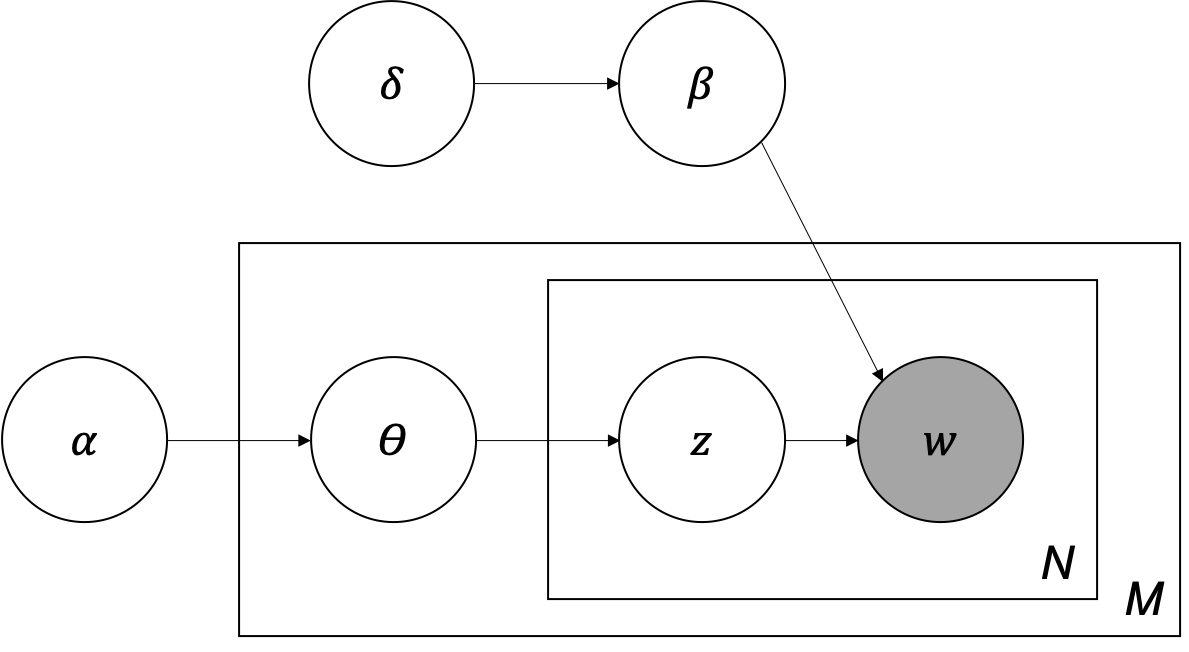
\includegraphics[width=0.5\textwidth]{LDA_Plate_Diagram.png}
	\caption{The well-established plate diagram for the standard LDA model extended by the parameter $\delta$. The slightly bigger box represents the generative model of the corporis $M$ documents. The smaller plate represents the iterative generation process of the $N$ words of each document with the aid of the topics. See also "smoothed LDA model" in \cite{Blei2003}  for comparisons.}
	\label{fig:PlateDiagram}
\end{figure}
\ \\
In order to estimate the model parameters, the first task is to calculate the posterior distribution, which consists of the joint distribution in the numerator and the marginal distribution in the denominator.

\begin{align}\label{posterior}
p(\theta,\textbf{z}|\textbf{w},\alpha,\beta)= \frac{p(\theta,\textbf{z},\textbf{w}|\alpha,\beta)}
{p(\textbf{w}|\alpha, \beta)}
\end{align}
The joint distribution numerator can be derived straight forward.

\begin{align}\label{joint}
p(\theta,\textbf{z},\textbf{w}|\alpha,\beta)=p(\theta|\alpha)\prod_{i=1}^{N}p(w_i|z_i,\beta)\ p(z_i|\theta)
\end{align}
One can obtain the marginal distribution of a document $\textbf{w}$, by integrating out the parameter $\theta$ and summing over the topics $z_j$. Nevertheless, this expression is intractable.
\begin{align}\label{marginal}
p(\textbf{w}|\alpha, \beta)=\int p(\theta|\alpha) \left( \prod_{i=1}^{N} \sum_{z_i}p(z_i|\theta)p(w_n|z_i,\beta) \right) d\theta
\end{align}
\ \\
The literature divides the approaches to calculating posterior distribution into two main categories.\cite{Blei2012} distinguishes between sampling based algorithms and variational algorithms. \cite{Powieser2012} lists a total of 6 algorithms that can be used to estimate parameters in the LDA model. This thesis will be confined to the two most cited and most used members of the two main groups. One approach is to simulate the posterior density by iteratively sampling - the so-called Gibbs sampling. The second approach is a deterministic method, a modified version of the well-known EM algorithm \cite{Dempster1977}: the Variational EM algorithm (VEM algorithm) \cite{Wainwright2008}. In the following two sections the both approaches are roughly outlined to give the reader some insight into the Bayesian inference underlying the algorithms.

\subsubsection{Variational EM algorithm}

In the VEM algorithm for the LDA model is a mean field approach which varies the steps E and M of the EM algorithm in a way such that this algorithm becomes solvable. Note that the main problem of calculating the marginal distribution is, to derive the conditional probability of some hidden variables given some observed values ("evidence"). The variation of the EM algorithms consists mainly in approximating the directly intractable E step.  Rewriting the log of the border density of $\textbf{w}$ as follows in (\ref{marginal2}), results in the fact that the marginal density can be estimated downwards with the aid of Jensen's inequality.
\begin{align}\label{marginal2}
\log p(\textbf{w}|\alpha, \beta) &= \log \int \sum_{z} 
p(\theta,\textbf{z},\textbf{w}|\alpha,\beta)d\theta\\
& =\log \int \sum_{z} \frac{p(\theta,\textbf{z},\textbf{w}|\alpha,\beta) q(\theta,\textbf{z})}{q(\theta,\textbf{z})}d\theta\\
&\geq \int \sum_{z} q(\theta,\textbf{z})\log p(\theta,\textbf{z},\textbf{w}|\alpha,\beta) d\theta - 
\int \sum_{z} q(\theta,\textbf{z})\log q(\theta,\textbf{z})d\theta\\
&= \mathbb{E}_q[\log p(\theta,\textbf{z},\textbf{w}|\alpha,\beta) ]-
\mathbb{E}_q[\log q(\theta,\textbf{z})] \label{KL}
\end{align}
Here $q(\theta,\textbf{z})$ is an arbitrary distribution which can be called the variational distribution. 
\begin{align}
q(\theta,\textbf{z})\widehat{=}q(\theta,\textbf{z}|\gamma,\phi)
=q(\theta|\gamma) \prod_{i=1}^N q(z_i|\phi_i)
\end{align}
The right hand side $L(\gamma,\phi,\alpha, \beta):=\mathbb{E}_q[\log p(\theta,\textbf{z},\textbf{w}|\alpha,\beta) ]-
\mathbb{E}_q[\log q(\theta,\textbf{z})]$ be called "lower bound". It can be shown that $\log p(\textbf{w}|\alpha, \beta) - L(\gamma,\phi,\alpha, \beta)$ is the Kullbak Leibler divergence ($D_{KL}$) of the true posterior and the variational distribution. From equations (\ref{marginal2})-(\ref{KL}) follows that:
\begin{align}\label{equality}
\log p(\textbf{w}|\alpha, \beta)= D_{KL}(q(\theta,\textbf{z}|\gamma,\phi)||p(\theta,\textbf{z},\textbf{w}|\alpha,\beta)) + L(\gamma,\phi,\alpha, \beta)
\end{align}
Since the marginal is fixed, we conclude, that minimizing the KL-divergence is equivalent to maximizing the lower bound (see \cite{Jordan1999} and \cite{Wainwright2008}, for details of the derivation of the lower bound see \cite{Blei2003}).
\begin{align}
(\gamma^*, \phi^*) &= \argmin_{\gamma, \phi}D_{KL}(q(\theta,\textbf{z}|\gamma,\phi)||p(\theta,\textbf{z},\textbf{w}|\alpha,\beta))\\
&= \argmax_{\gamma, \phi} L(\gamma,\phi,\alpha, \beta)
\end{align}\\
\\
The variation of the EM algorithm thus is to use the variational distribution $q(\theta,\textbf{z}|\gamma^*(\textbf{w}), \phi^*(\textbf{w}))$ instead the posterior distribution $p(\theta,\textbf{z},\textbf{w}|\alpha,\beta)$. Now the two steps of the VEM algorithm are:
\begin{itemize}
	\item [(1)]\textbf{E step} Optimize the variational parameters $\theta$ and $\phi$ for every document in the corpus. This can be done analytically by deriving the derivatives of the KL divergence. And set them to zero.
	\item [(2)] \textbf{M Step} Maximize the lower bound using the optimized parameter of the E step with respect to $\alpha$ and $\beta$.
\end{itemize}


\subsubsection{Gibbs sampling}

The second method to approximate the posterior distribution is Gibbs sampling, a so-called monte Carlo method. Instead of calculating the distributions for $\beta$ and $\theta$, the primary task is to find the posterior distribution over $\textbf{z}$ given the document $\textbf{w}$. Gibbs sampling is also known as a Markov Chain Monte Carlo method. The name refers to the simulation process by which a chain of values is simulated whose limiting distribution desirably converges against the true distribution \cite{Griffiths2006}. (\ref{Gibbs}) shows the distribution, which is sampled from iteratively.
\begin{align}\label{Gibbs}
p(z_i=j|z_{-i},w)\propto \frac{n_{-i,j}^{(l)}+\delta}{\sum_t n_{-i,j}^{(t)}+V\delta}
\frac{n_{-i,j}^{(d_i)+\alpha}}{n_{-i}^{(d_i)}+k\alpha}
\end{align}
\makebox[1cm][l]{$z_{i}=j$} 		... \makebox[5cm][l]{word-topic assignment of word $i$ to topic $j$}\\
\makebox[1cm][l]{$z_{-i}$}   		... \makebox[4cm][l]{vector of word-topic assignments without the entry for word $i$}\\
\makebox[1cm][l]{$n_{-i,j}^{(l)}$}	... \makebox[4cm][l]{number of times the $l$th word in the vocabulary is assigned to }\\
\makebox[1cm][l]{}						\makebox[4cm][l]{\ \ \ \ topic $j$, not including the assignment for word $i$}\\
\makebox[1cm][l]{$d_i$}				... \makebox[4cm][l]{document in the corpus which includes word $i$}\\
\makebox[1cm][l]{$\delta,\alpha$} 	... \makebox[4cm][l]{parameters of the prior distributions for $\beta$ and $\theta$}\\
\\
Usually the word-topic distributions $\beta_{j}^{(l)}$ for the words $l=1,...,V$ and topics $j=1,..,k$ and topic-document distributions $\theta_j^{(d)}$ for the documents $d=1,...,D$ and the topics $j=1,...,k$ will be of interest. (\ref{Gibbs:beta}) and (\ref{Gibbs:theta}) shows the predictive distributions denoted as "estimators". 
\begin{align}
\hat\beta_{j}^{(l)}&=\frac{n_{-i,j}^{(l)}+\delta}{\sum_t n_{-i,j}^{(t)}+V\delta} \label{Gibbs:beta} \\
\hat\theta_j^{(d)}&= \frac{n_{-i,j}^{(d_i)+\alpha}}{n_{-i}^{(d_i)}+k\alpha} \label{Gibbs:theta}
\end{align}
For derivation and more details regarding the Gibbs sampling procedure see \cite{Griffiths2006}.

\subsubsection{Implementation}

In this thesis, the implementation of the LDA model and its estimation is mainly based on using the package \texttt{topicmodels} of Kurt Hornik. The package \texttt{topicmodels} can apply both the VEM algorithm as well as Gibbs sampling in order to fit the model. In addition, the package \texttt{tidytext} is being used for text structuring and embedding. Whereby there are other packages besides this implementation of the LDA model, \texttt{topicmodels} is particularly convenient, because \texttt{tidytext} was designed by its developers to work perfectly in combination with \texttt{topicmodels} \cite[p. 89]{Silge2017}.


\subsection{Artifical Neural Networks}

Artificial neural networks (ANN) are much more versatile than the LDA model. There are not only various forms of artificial neural networks, but also a very large number of application areas. Quite as machine learning procedures in general, also deep learning algorithms are divided into two broad categories: supervised learning, where a superset instance provides the algorithm with the output required to learn, and unsupervised procedures that internally train predefined models to find patterns in the input signals. In this chapter we will focus heavily on the former group of ANNs. Also, this chapter is intended to give the reader an overview of the research on neural networks as well as the background of their development. \\
\subsubsection{Development}
Research on ANNs dates back to the 1940s, when \cite{McCulloch1943} introduced the so called “M-P neuron”. Whereby this neuron had only a bivariate input and output, Rosenblatt later extended this idea to a network of M-P neurons, which allowed to set up a simple classification algorithm \cite{Rb1958}. A perceptron in its basic form (single perceptron) is a binary classifier. \\
\\
Imagine input data of a simple perceptron in the form of a matrix. 
$$X= \left[
\begin{array}{rrr}                                
x_{11} & \dots & x_{1k} \\                                               
\vdots & \ddots & \vdots \\                                               
x_{n1} & \dots & x_{nn} \\                                             
\end{array}
\right] = \left[
\begin{array}{r}                                
\textbf{x}_{1} \\                                               
\vdots \\                                               
\textbf{x}_{n} \\                                             
\end{array}
\right]
$$ 
The dependent variable thus is a vector $\textbf{y}=y_1,…,y_n$, with $y_i\in \{0,1\}$. Consider the lines of the X mtrix as vectors $\textbf{x}_1,…,\textbf{x}_n$, with $\textbf{x}_i\in\mathbb{R}^k$. The entries of each of the vectors are weighted with $\textbf{w}=w_1,\dots,w_k$ with $w_j \in \mathbb{R}$ and aggregated in a function $h$ e.g. a sum.
$$h(\textbf{x},\textbf{w})=\sum_{j=1}^kx_jw_j$$
Using a so called "activation function" $h$ is mapped to the output space, which is in this case $O=\{0,1\}$. At this point a step function serves as activation function.
$$a \circ h(\textbf{x},\textbf{w}) = \begin{cases} 0 \text{ if } h(\textbf{x},\textbf{w}) \leq 0 \\ 1 \text{ else}\end{cases}$$
The matrix $X$ is passed vector by vector to the percepron and the output is compared with the values for $\textbf{y}$. During this procedure the weights are iteratively tuned by a simple updating algorithm using the pairs $\textbf{x}_i$ and $y_i.$

\begin{figure}[h]
	\centering
	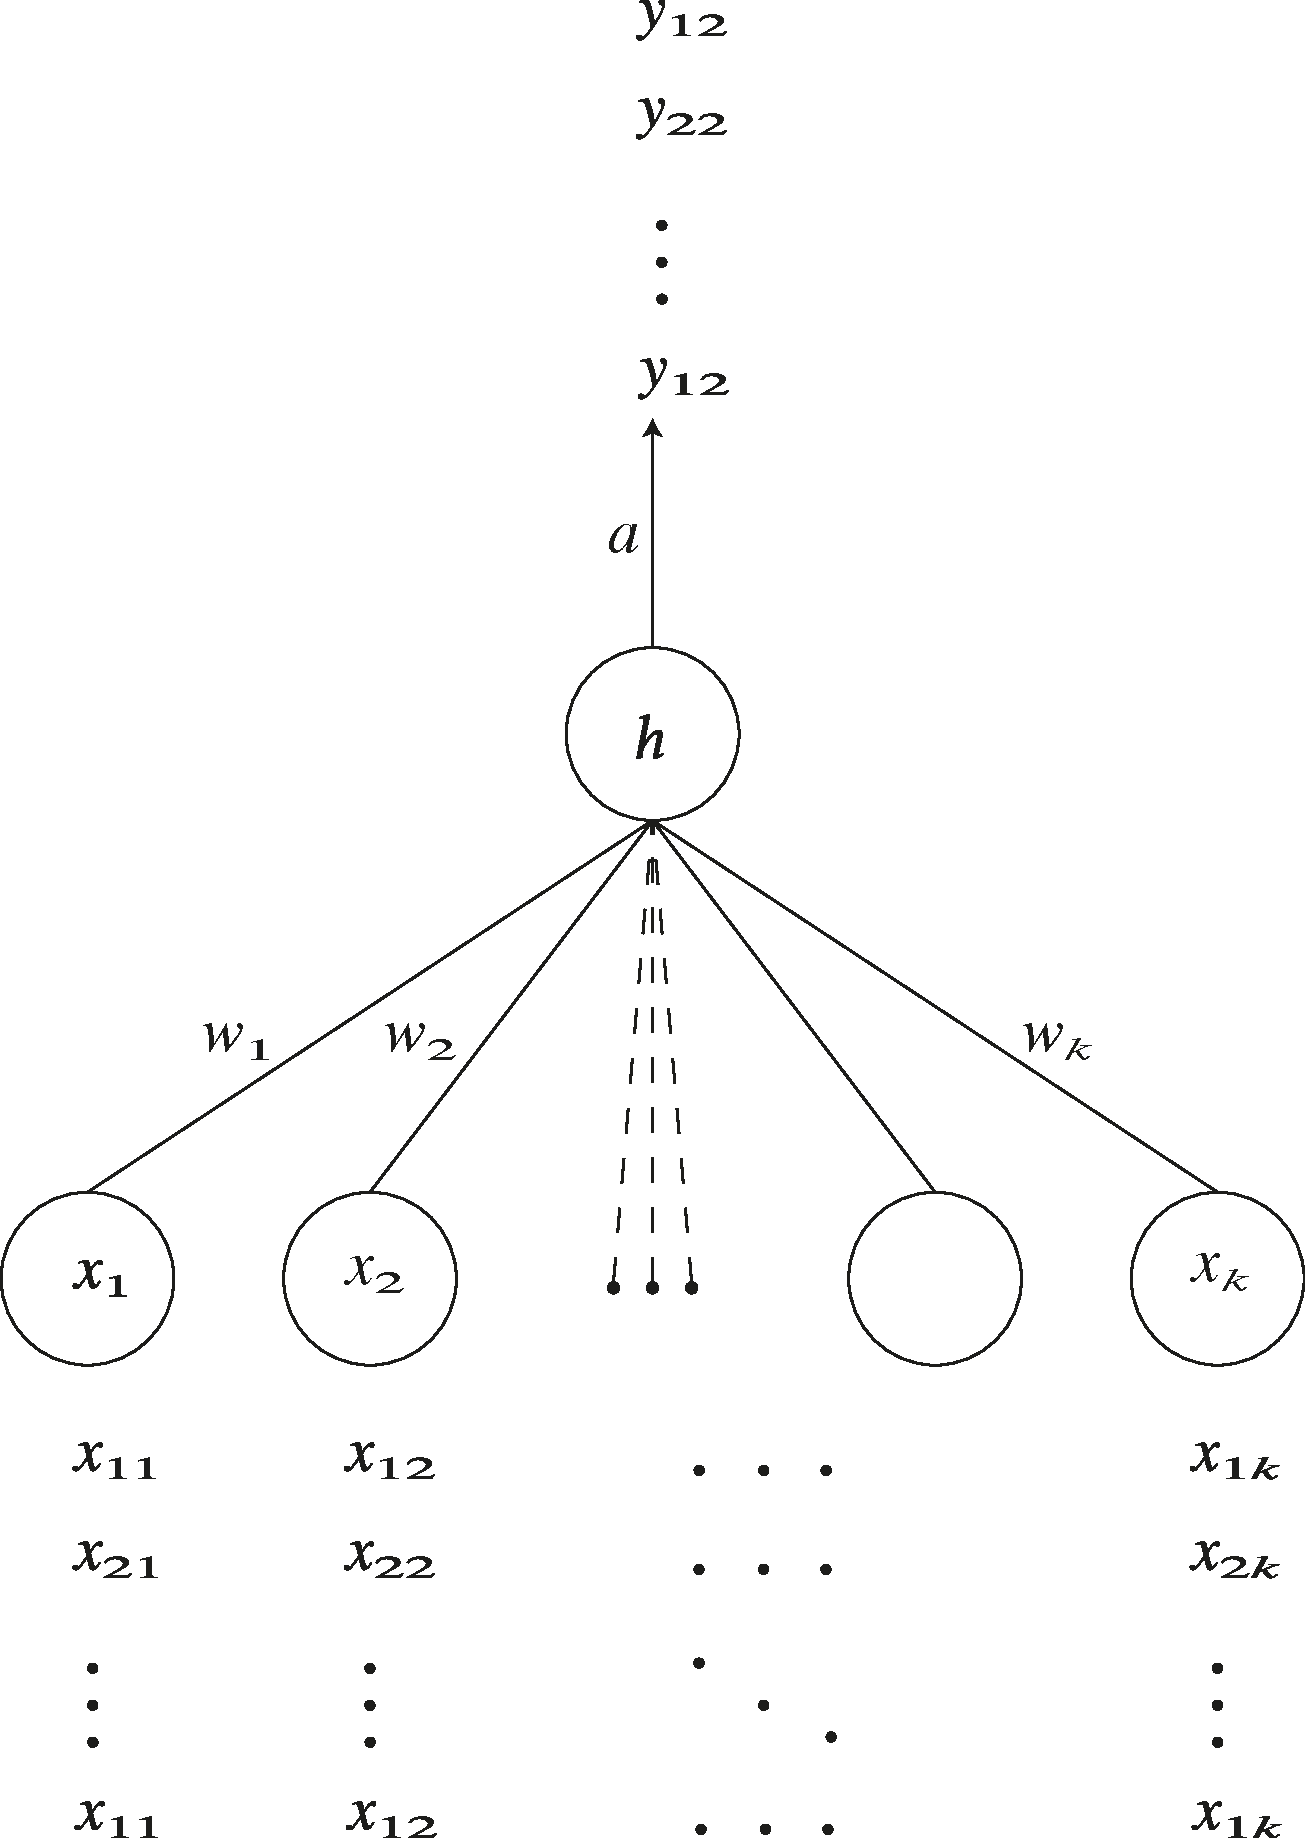
\includegraphics[scale=0.4]{simple_perceptron.pdf}
	\caption{Schematic diagram of a simple perceptron by \cite{Rb1958}}
	\label{simple_perceptron}
\end{figure}
\ \\
The algorithm of the simple perceptron is schematically shown in Figure \ref{simple_perceptron}. This diagram corresponds to the common representation in education \cite{Mekherjee2019}, although a horizontal perspective is often chosen.\\
\\
If this basic perceptron is used in a clever way, designs can be developed that have variable application possibilities with this approach only. For example, a sigmoid function can be used as an activation function instead of the step function. So the output layer will not project into the $\{0,1\}$ space, but into a probability space. If you add several nodes with the sigmoid activation function rather than a single output, you basically obtain the architecture that is also called multivariate logistic regression \cite{Bahjat2006}. In that case the model can be estimated by an individual calculation of logistic regressions for each node in the output layer. This allows to classify not only two classes, but an arbitrary number (see the network architecture of Figure \ref{adaption_perceptron}). \footnote{Note that in this setting the dependent variable must be one-hot encoded.}\\
\begin{figure}[h]
	\centering
	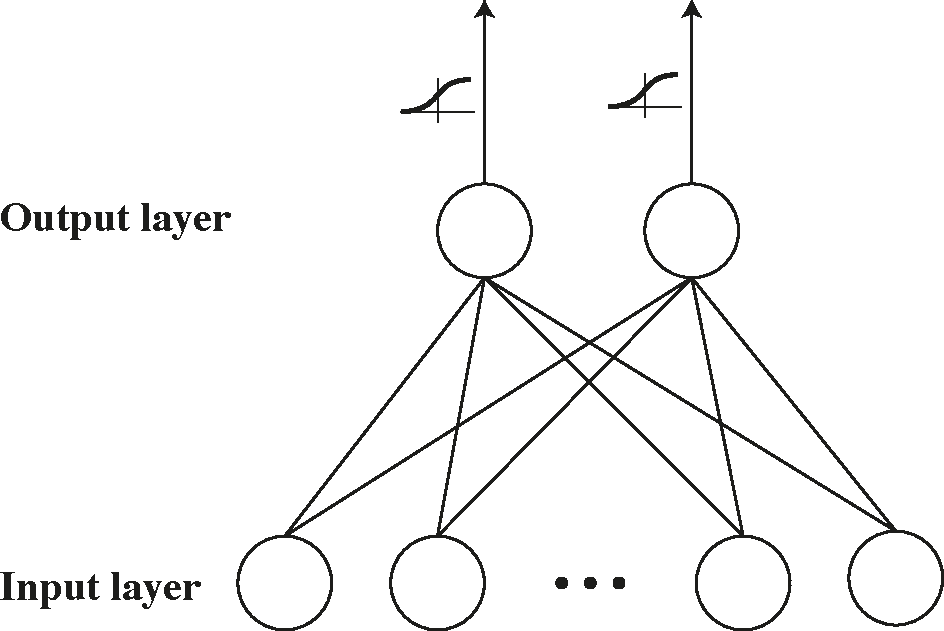
\includegraphics[scale=0.5]{adaption_perceptron.pdf}
	\caption{Schematic diagram of an adapted Rosenblatt-perceptron network}
	\label{adaption_perceptron}
\end{figure}
\ \\
Shortly following the publication of these results, which would lay the foundation for later neural networks, ANN research had to suffer a severe setback after Minsky and Papert \cite{Minsky1969} were able to prove that perceptrons cannot provide a suitable solution in certain basic scenarios. It is possible to separate two clusters by a hyperplane with the perceptron, however, if the two groups could not be separated completely, the perceptron failed. For instance, it was impossible to find a solution for data generated with an \textit{x-or} function (also called "exclusive or" function).\\
\ \\
Although the researchers Minsky and Papert showed that the perceptron in this form cannot solve the “xor problem”, they argued that extending the simple perceptron to a multi layer perceptron is an approach to solve this problem, if it was feasible to train this model. Instead of just one input layer and one output layer, an MLP may include an arbitrary number of hidden layers in between. Figure \ref{figure:MLP} shows the structure of such an network. However, with the naive optimizing algorithm of the perceptron as it was designed by Rosenblatt, it was not feasible training a model with an architecture of that kind.\\
\begin{figure}[h]
	\centering
	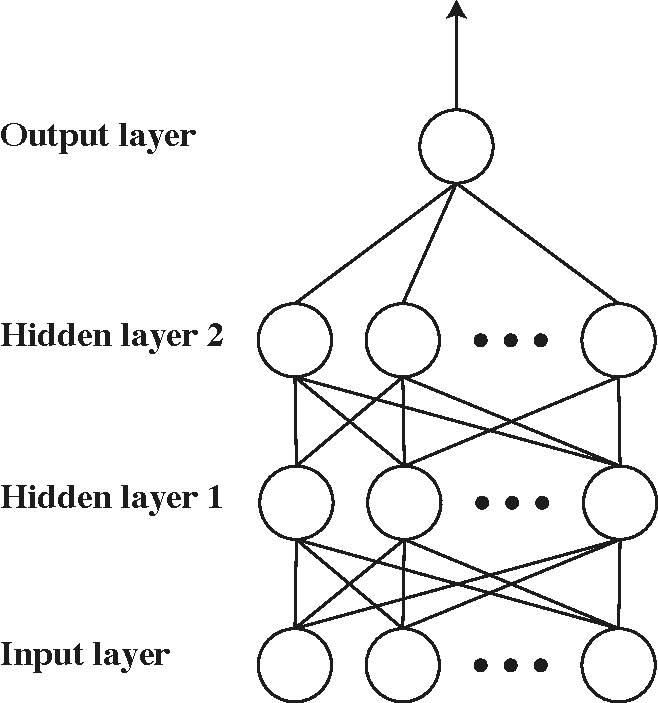
\includegraphics[scale=0.6]{MLP.pdf}
	\caption{Schematic diagram of an multi layer perceptron (MLP)}
	\label{figure:MLP}
\end{figure}
\ \\
\subsubsection{Backpropagation}
The procedure used to optimize the weights of a multilayer perceptron is called backpropagation. This method was first applied to neural networks by Webos - as part of his dissertation \cite{Werbos1974}- and still works the same way to this day. It is important to use a sigmoid function instead of the step function which is used in the perceptron, as this function is differentiable.  Assume a random initial distribution of the weights $w_1,\dots,w_d$ for a network with $d$ layers, which are the starting values for the update procedure. Let $\tau_i$ be the number of units in layer $i$. So layer $i$ can be denoted as function $f_{w_i}$ and the whole network as a chain of functions.
\begin{align}\label{network_chain}
	\hat{y_i}=f_{w_d}(f_{w_{d-1}}(...(f_{w_1}(x_i))))=f_{w_d}\circ f_{w_{d-1}} \circ \dots \circ f_{w_1}(x_i)
\end{align}
The goal is to update the weights of each layer in sucha way as to minimise a selected loss function $L(w_1,\dots,w_d)$. A common loss function is for example quadratic loss: $L=\frac{1}{2}\sum_{i=1}^n(\hat{y_i}-y_i)^2$\\
The backpropagation algorithm consist of the 3 following roughly outlined steps.
\begin{enumerate}
	\item \textbf{forward pass:} Calculation of the result $y_i$ for all units at the set weights
	\item \textbf{backward-sweep:} Each layer's derivatives are now calculated using the chain rule, step by step - starting with the output layer. For the output layer this is:
	\[\frac{\partial L}{\partial w_d}=\frac{\partial L}{\partial f_d(x_i)}\frac{\partial f_d(x_i)}{\partial w_d}	\]
	\item \textbf{updating:} Update the weights by an arbitrary optimization algorithm. E.g. steepest descent:
	$\Delta w_d=\alpha \frac{\partial L}{\partial w_d}$
	,where $\alpha$ is the learning rate
\end{enumerate}
Thanks to current software, the derivatives no longer have to be calculated for each node by hand, but the standard packages are capable of "symbolic differentiation" for certain network structures, which makes training neural networks comfortable \cite[p. 47]{Chollet2018}.\\
\ \\
Note: While Rosenblatt for the perceptron was actually inspired by the biological structure of the neurons in the brain, more complex “networks used by engineers are only loosely based upon biology”\cite{Hecht-Nielsen1988}.

\subsubsection{Implementation}
This work uses the \texttt{Keras R} package to create neural networks, a deep learning API (Application-Programming-Interfac) to deep learning backend engines, designed for \texttt{R} by Allaire in 2017. Keras is a so called “model-level” library, designed to set up complex neural net architectures using well arranged, high-level building blocks. As backend-engine the users are provided with TensorFlow, Theano and Microsoft Cognitive Toolkit. Using these backend engines computation may be processed seamlessly via CPU or GPU \cite{Chollet2018}.

% ANALYSIS OF TEXTBOOK CHAPTERS
\section{Analysis of textbook chapters}\label{sec:analysis}

In this first example, the chapters of individual books are classified, all of which sourced from the freely distributed Project Gutenberg. Project Gutenberg is a provider of over 60,000 free electronic books with the primary aim to “encourage the creation and distribution of eBooks”\cite{ProjectGutenberg}. The package \texttt{gutenbergr} \cite{gutenbergr} preprocesses the ebooks text data and downloads it. This convenient package in combination with the free repository allows the analysis of a large number of large text documents with a secure source and a big amount of meta information. For this analysis interesting information is e.g. Gutenberg id as key variable for fast identification of books, title, author and more importantly the categorization of project Gutenberg, the so-called Gutenberg bookshelf. Table \ref{titles:5books} lists all this information for a random sample of books downloaded from the Project Gutenberg.

\begin{table}[!htbp] \centering 
	\caption{Example book corpus} 
	\label{titles:5books} 
	\tiny
	\begin{tabular}{@{\extracolsep{2pt}} c|c|c|c} 
		\hline 
		\hline \\[-1.8ex] 
		gutenb. id & title & author & gutenberg bookshelf \\ 
		\hline \\[-1.8ex] 
		$2095$ & Clotelle: A Tale of the Southern States & Brown, William & African American Writers \\ 
		$6315$ & The Awakening of Helena Richie & Deland, Margaret & Bestsellers, American\\ 
		$6971$ & Judaism & Abrahams, Israel & Judaism \\ 
		$7635$ & The Disowned — Volume 05 & Lytton, Edward and Baron & Historical Fiction \\ 
		$10319$ & Dave Darrin's Third Year at Annapolis & Hancock, Harrie Irving & Children's Book Series \\
		\hline 
	\end{tabular} 
\end{table} 
\ \\
In order to test NLP models, two questions can be examined on the basis of these simple text documents. 
\textbf{Firstly (Q1), does a clustering model cluster text documents similar to a human-driven classification?} In this case, this could be validated by the categorization into Gutenberg bookshelves. \textbf{And secondly (Q2), how good is such a classification reproducible using a classification model?} \\
Since very large amounts of data have to be processed and analyzed in order to model the bookshelf classification for a big collection of books, a somewhat reduced approach will be used here. One breaks down a collection of books of different categories into chapters in order to cluster respectively classify these chapters as independent documents. Similarly, you could give an example, assuming $N$ books and separate their chapters and shuffle them, is it possible to use models to reassemble the chapters into stacks that can be assigned to individual books?\\
\ \\
The raw text record is now transformed into the tidy format of tidytext (i.e. one word per row). Now it is possible to remove unnecessary stop-words. These words are predefined and can be modified for the appropriate use case if necessary. The words stem from 3 sources, "onix", "SMART" and "snowball", whereas the latter two are pulled from the \texttt{tm} package \cite{tidytext}.  And the Onix stop words are taken from the publicly accessible site lextec.com. An example of stop words can be found in Table \ref{stopwords}.
\begin{table}[!htbp] \centering 
	\footnotesize
	\caption{Example of stop words from tidytext package} 
	\label{stopwords} 
	\begin{tabular}{@{\extracolsep{5pt}} cc} 
		\\[-1.8ex]\hline 
		\hline \\[-1.8ex] 
		word & lexicon \\ 
		\hline \\[-1.8ex] 
		many & SMART \\ 
		mrs & onix \\ 
		was & snowball \\ 
		sure & onix \\ 
		you're & snowball \\ 
		go & onix \\ 
		c & SMART \\  
		where & snowball \\ 
		then & SMART \\ 
		\hline \\[-1.8ex] 
	\end{tabular} 
\end{table} 
\\
Both models that are studied in this thesis, use a bag of words data set as input data. This means a matrix with the documents in the $M$ lines and the frequencies of the $V$ used words in the entries of the columns. The dimension - i.e. the number of words in this "dictionary" $V$ - may be reduced for two reasons. For one thing, a dimension reduction can reduce the fitting time of the model, for another thing, the diversity of the documents can be increased by skilfully reducing certain words, which occur equally frequently in all documents. Now this requires a special measure on which we decide which words to exclude. One can call this reduction of the bag of words dimensionality "embedding". In the course of this work 3 different embedding methods were tested. 
\begin{enumerate}
	 \item The reduction by the words that occur with a low frequency. 
	\item No dimension reduction, i.e. use of the full dictionary of all occurring words. 
	\item The reduction with the aid of the measure \textit{tf-idf}.
\end{enumerate}

\textit{tf-idf} is a combination of the term frequency and the inverse document frequency, defined as follows.
$$\text{\textit{tf-idf}}(t,d):=tf(t,d)\times idf(t)$$
$$tf(t,d):=\frac{f_{t,d}}{\sum_{t_i=1}^V f_{t_i,d}}$$
$$idf(t):=\ln\left(\frac{M}{n_{d'\in t}}\right)$$
\\
\makebox[1cm][l]{$t$} 		... \makebox[5cm][l]{term (word)}\\
\makebox[1cm][l]{$d$}   	... \makebox[4cm][l]{document}\\
\makebox[1cm][l]{$f_{t,d}$} ... \makebox[4cm][l]{frequency of term $t$ in document $d$}\\
\makebox[1cm][l]{$M$} 		... \makebox[5cm][l]{number of documents}\\
\makebox[1cm][l]{$n_{d'\in t}$}   	... \makebox[4cm][l]{number of documents containing term $t$}

\ \\
Even if “its theoretical foundations are considered less than firm by information theory experts”, \textit{tf-idf} “has proved useful in text mining” \cite{Silge2017}. In this thesis the term frequency and the \textit{tf-idf} are not to be used directly for the analysis of the texts but mainly for setting up the bag-of-words datasets. It shall be investigated whether the use of different embeddings has an influence on the text analysis itself.

% SUBSECTION
% Lda applied on Gutenberg Data
\subsection{LDA applied on Gutenberg data}

As LDA is a classification algorithm, the research question Q1 should be addressed first. I.e. to what extent does the clustering of the LDA model correspond to the mapping of chapters to books? In the first attempt only 6 books are sampled. That is, there are 6 categories, because as mentioned in \ref{sec:analysis} all these 6 books were taken from different bookshelves.\\
\ \\
As described in Chapter \ref{sec:LDA}, it is possible to calculate the LDA model by means of two different algorithms. These are the VEM algorithm and Gibbs sampling. In this study we examined both methods. Clearly, the algorithms may differ in the speed of the calculation. However, it does not have to be the case that both calculation methods deliver the same results.\\
\ \\
Three fundamentally different approaches should be distinguished for embedding:
\begin{enumerate}
	\item the entire dictionary, i.e. all words occurring in the corpus are used for the bag of words.	
	\item for the bag of words only words are used which occur at least 2 times in the whole corpus. This reduces the number of used words and therefore the dimension of the data by nearly 50\%.
	\item the bag of words is reduced by the same amount as in case two, but not according to absolute frequency, but according to \textit{tf-idf}.
\end{enumerate}
These approaches are reviewed with regard to the goodness of the fit and the speed of the computation. One intuitively may assume that the calculation takes longer for data with higher dimensionality.\\
\ \\
For a clustering model there are two useful methods to evaluate the fit. On the one hand it is possible to fit the model with training data and to evaluate the goodness of the fit using the test data. On the other hand, it is a comparison of the classification of the model with the categories given by the data, whereby the model does not learn from these categories. The latter evaluation method is clearly less computationally intensive, and the comparison of the entire data set instead of only the test part of the data has a positive effect on the variance. Starting this analysis the second approach is used primarily.\\
\ \\
The findings of this study relating to the LDA model are documented in detail. You will find the documentation regarding the LDA model as well as the other models in the appendix. For the sake of clarity, a separate document with the corresponding results was created for each analyzed example and each model respectively. To ensure reproducibility, the entire code is attached to the work by means of these documentations, and will be published on GitHub as well.\footnote{\url{https://github.com/SebastianKnigge/Master_Thesis/tree/master/Documentations} }\\
\ \\
The computation of the LDA model via VEM takes a somewhat longer time in the two samples evaluated. In all cases investigated, i.e. across the two samples taken and for both VEM and Gibbs sampling, the calculation for the tf-idf embedding appeared to be the fastest. The calculation time for embedding according to term frequency and full embedding differs less and the calculation of the term frequency embedding is not faster in every case. While a reduction via term frequency only cuts the most rarely used words, a reduction via tf-idf also cuts out frequent words as long as they occur frequently in all documents. Thus the tf-idf reduction has more impact on the distribution within each document compared to the effect of the term frequency reduction, which only affects the tails of the marginal distribution. This supports the assumption that a higher degree of difference in the documents has a positive effect on the calculation speed. 









\newpage 
.
\newpage
\appendix
\section{Appendix}
	
  \bibliographystyle{apalike}
  \bibliography{MagLibrary}


\listoffigures
\listoftables

	
	
\end{document}